\section{Source Code Information}

\figref{code_lines} shows the size of the kernels in terms of lines of code. The average number of lines of code for the $752$ kernels in the evaluation set was $17.67$, and the median was $11$. $14$ kernels had more than $100$ lines of code, and $47$ had more than $50$ lines of code. $50\%$ of the kernels had less than $25$ lines of code. The kernel with the highest number of lines of code had $639$ lines.

\begin{figure}[htp]
\centering

\begin{minipage}{.45\textwidth}
    \centering
    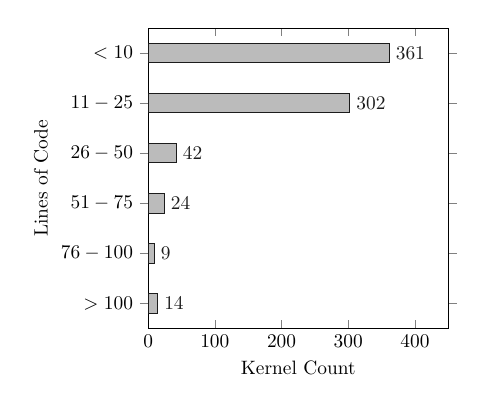
\begin{tikzpicture}[scale=0.7]
    
    \selectcolormodel{gray}
    
    \begin{axis}[
        xbar, xmin=0, xmax=450,
        xlabel={Kernel Count},
        symbolic y coords={
            {$> 100$},
            {$76-100$},
            {$51-75$},
            {$26-50$},
            {$11-25$},
            {$< 10$}
        },
        ytick=data,
        ylabel={Lines of Code},
        nodes near coords,
        nodes near coords align={horizontal},
        height=200pt, width=200pt
    ]
    
    \addplot coordinates {
        (14,{$> 100$})
        (9,{$76-100$})
        (24,{$51-75$})
        (42,{$26-50$})
        (302,{$11-25$})
        (361,{$< 10$})
    };
    
    \end{axis}
    \end{tikzpicture}
    
    \caption{Lines of Code}
    \label{Fi:code_lines}
\end{minipage}
\hfil
\begin{minipage}{.5\textwidth}
    \centering
    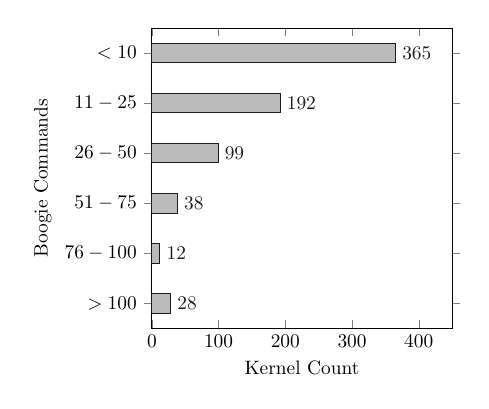
\begin{tikzpicture}[scale=0.7]
    
    \selectcolormodel{gray}
    
    \begin{axis}[
        xbar, xmin=0, xmax=450,
        xlabel={Kernel Count},
        symbolic y coords={
            {$> 100$},
            {$76-100$},
            {$51-75$},
            {$26-50$},
            {$11-25$},
            {$< 10$}
        },
        ytick=data,
        ylabel={Boogie Commands},
        nodes near coords,
        nodes near coords align={horizontal},
        height=200pt, width=200pt
    ]
    
    \addplot coordinates {
        (28,{$> 100$})
        (12,{$76-100$})
        (38,{$51-75$})
        (99,{$26-50$})
        (192,{$11-25$})
        (365,{$< 10$})
    };
    
    \end{axis}
    \end{tikzpicture}
    
    \caption{Boogie Commands}
    \label{Fi:boogie_commands}
\end{minipage}

\end{figure}


It should be noted that the instrumentation step of \tool happens on the Boogie code and not on the source code. A line of code in the source file could result in no Boogie commands (e.g., code comments) or more than one Boogie command (e.g., multiple assignments on a single line). \figref{boogie_commands} shows the size of the kernels in terms of Boogie commands. The average number of Boogie commands for the $734$ kernels for which Boogie code was generated was $25.72$, and the median was $11$. $50\%$ of the kernels had less than $25$ commands. The kernel with the highest number of Boogie commands had $1793$ commands.

\begin{figure}[htp]
\centering

\begin{minipage}{.45\textwidth}
    \centering
    \begin{tikzpicture}[scale=0.7]
    
    \selectcolormodel{gray}
    
    \begin{axis}[
        xbar, xmin=0, xmax=300,
        xlabel={Kernel Count},
        symbolic y coords={
            {$> 100$},
            {$21-100$},
            {$11-20$},
            {$6-10$},
            {$4-5$},
            $3$,
            $2$,
            $1$,
            $0$
        },
        ytick=data,
        ylabel={Barrier Count},
        nodes near coords,
        nodes near coords align={horizontal},
        height=200pt, width=200pt
    ]
    
    \addplot coordinates {
        (@@barriers_inf@@,{$> 100$})
        (@@barriers_100@@,{$21-100$})
        (@@barriers_20@@,{$11-20$})
        (@@barriers_10@@,{$6-10$})
        (@@barriers_5@@,{$4-5$})
        (@@barriers_3@@,$3$)
        (@@barriers_2@@,$2$)
        (@@barriers_1@@,$1$)
        (@@barriers_0@@,$0$)
    };
    
    \end{axis}
    \end{tikzpicture}
    
    \caption{Kernels with 'n' Instrumented Barriers}
    \label{Fi:kernels_barriers}
\end{minipage}

\end{figure}


The repair step of \tool does not depend on the number of lines or code nor the number of Boogie commands. It depends on the number of barriers that are instrumented in code which depend on the number of shared variables and how many times they have been used.

\figref{kernels_barriers} shows the number of barrier variables introduced in the instrumentation stage of \tool. This also includes the barrier variables introduced for existing barriers provided by the programmer. Out of the $734$ kernels that reached the instrumentation stage (inclusive of CUDA and OpenCL kernels), for $50\%$ of the kernels, the number of instrumented barriers introduced were less than or equal to $3$, whereas, there were $5$ kernels with more than $100$ instrumented barriers. For $50\%$ of the kernels, the time taken by the instrumentation stage of \tool was less than a second.
